\documentclass[11pt]{article}

\usepackage[latin1]{inputenc}
\usepackage{amsmath,amsthm,amssymb}
\usepackage{graphicx}

\usepackage{pdfsync}
\usepackage{epsfig}
\usepackage{epstopdf}
\usepackage{mystyle}


% format A4
\usepackage{vmargin}
\setpapersize{A4} 


% for the display of algorihtms
\usepackage[ruled,vlined]{algorithm2e}
\usepackage{float}
\floatstyle{boxed}
\floatstyle{ruled}
\newfloat{listing}{H}{loi}
\floatname{listing}{Table}


\graphicspath{{./images/}}


\title {A Projection Approach to the Numerical Analysis\\of Limit Load Problems}

\author{Guillaume Carlier \\\small CEREMADE \\\small Universit\'e Paris Dauphine
                \\\small \tt carlier@ceremade.dauphine.fr \and  
     	Myriam Comte\\\small Laboratoire Jacques-Louis Lions, \\\small Universit\'{e} Pierre et Marie Curie 
				\\\small \tt comte@ann.jussieu.fr \and 
       	Ioan R. Ionescu \\\small LPMTM  \\\small Universit\'e Paris 13
                \\\small \tt ioan.r.ionescu@gmail.com \and
        Gabriel Peyr\'e \\\small CEREMADE \\\small Universit\'e Paris Dauphine
                \\\small \tt peyre@ceremade.dauphine.fr
}

% GP : je crois qu'il faut des majuscule � tous les mots des titres de section en anglais.


%GC: non ce n est pas une regle absolue meme si beaucoup d auteurs le font, laissons comme ca

%%%%%%%%%%%%%%%%%%%%%%%%%%%%%%%%
\begin{document}

\maketitle


\begin{abstract}
	This paper proposes a numerical scheme to approximate the solution of (vectorial) limit load problems.
	The method makes use of a strictly convex perturbation of the problem, which corresponds to 
	a projection of the deformation field under bounded deformation and incompressibility constraints.
	The discretized formulation of this perturbation converges to the solution of the original landslide problem when the amplitude of the perturbation tends to zero.	
	The projection is computed numerically with a multi-steps gradient descent on the dual formulation of the problem.
\end{abstract}

\textit{Keywords:} limit load analysis, functions of bounded deformation, penalizations, Nesterov algorithm.


%%%%%%%%%%%%%%%%%%%%%%%%%%%%%%%%%%%%%%%%%%%%%%%%%%%%%%%%%%%%%%%
%%%%%%%%%%%%%%%%%%%%%%%%%%%%%%%%%%%%%%%%%%%%%%%%%%%%%%%%%%%%%%%
%%%%%%%%%%%%%%%%%%%%%%%%%%%%%%%%%%%%%%%%%%%%%%%%%%%%%%%%%%%%%%%
\section{Introduction}

   Limit analysis, which  is the  simplest approach for modeling the inelastic response of structures, is based on a very idealized representation of a   rigid, perfectly plastic material subject to  slowly increasing loads.    The main problem in limit analysis is to find the maximum multiple of the force distribution that  the solid can withstand without collapsing.   Usually,  the  associated collapse flow field exhibits discontinuities on some surfaces and  the strain rates are bounded measures   (strain localization).  That is why, from both mathematical and numerical points of view,   limit analysis was and remains a difficult problem.   
   
   \smallskip
   
   The   numerical methods in limit analysis are based on the discretization of the kinematic or static variational principles (established in  \cite{DPG})    using  finite element method  techniques and on  convex and linear programming.  The first results were obtained in \cite{A,HM,HB}, while the literature on FE methods applied to limit analysis is very extensive (see for instance  \cite{ACO,Ch,CA,LS02,NPR,TN}).   Recently,  a new method, called  discontinuous velocity domain splitting   (DVDS) and originated in  \cite{lri} (see also \cite{hilr}), was proposed in \cite{IO}. DVDS  is a mesh free method which focuses on the strain localization and completely neglects the bulk deformations. 

	  \smallskip

 The goal  of this paper is to propose a new numerical technique for  the limit load problem, based on a projection with a specific  weighted  {L$^2$} norm.  Only the Von-Mises yield condition is considered  in this paper,  but the proposed  numerical method may,  in principle,   be extended  to other  plastic models.    The main idea  comes from a convergence result of a perturbed problem, obtained in \cite{buttazzo-cheeger} in the anti-place case, which selects the maximal collapse domain (called the Cheeger set  in a geometrical context  \cite{cheeg} and related to the  first eigenvalue of the degenerate 1-Laplacian operator  \cite{demg,kf}).    The associated numerical method was developed in \cite{carlier-cheeger-numeric}  using  a  finite difference discretization and a subgradient projection  iterative algorithm,   introduced in  \cite{combettes-pesquet-tv}. 
 
 	  \smallskip
 
 The Cheeger constant was introduced in \cite{cheeg} to  give a lower bound on the first eigenvalue of the Laplacian and  found a wide range of applications (denoising model in image processing, continuous max-flow/min-cut duality)   in recent years  \cite{rof,acc2, acc,strang1, strang2}.  For  convex domains, the uniqueness of the Cheeger set can be proved  \cite{ccn, ac}  and  explicit constructions (see \cite{klr}) are known in dimension two.  The connection between limit load analysis and the Cheeger problem  with weights  was established in \cite{lri, hilr} where various properties of the minimizers can be found.  The existence of Cheeger sets were proved,  but uniqueness does not hold in general which makes it difficult to compute numerically Cheeger sets. Fortunately, there is a unique maximal Cheeger set (see \cite{cc}) and it is proved in \cite{buttazzo-cheeger}  that it can be approximated by adding a small strictly convex penalization.  Starting from this penalization scheme, a convergent projection algorithm is implemented in \cite{carlier-cheeger-numeric}  to approximate maximal Cheeger sets. 
 
 
   \smallskip


Our aim in this paper is to generalize the strategy and the convergence results of \cite{carlier-cheeger-numeric} to handle the, physically more relevant, two-dimensional in-plane flow case that is detailed in the next paragraph.  The extension of the method proposed in  \cite{carlier-cheeger-numeric} for the anti-plane flow to the vectorial case of the in-plane or of 3-D problems is a difficult task.  It presents several additional difficulties, both from  theoretical and numerical points of view. First of all,  the  coarea formula  is not any more valid in  the vectorial case and the link  between the variational and  the geometrical problems is an open problem. Second,  we have to handle the divergence free condition and  the space of bonded deformations $\BD$ (instead of ${\rm{BV}}$), difficulties which   which are  not present in the anti-plane (scalar) case. 

\smallskip

Let us outline the content of the paper. In section 2, we give the  physical description of the limit load problem. The initial variational formulation is relaxed to get a good functional framework for the existence of  a solution.  In section 3, we introduce the anti-plane and in-plane cases. For the first of them (scalar case)  we recall the main  theoretical and numerical results,  needed to understand the approach  of the in-plane (vectorial) case developed in the remainder of the paper.   In section 4, we present the  penalization scheme. We prove  the   convergence  of the  penalization scheme  and the convergence for the discretized problems.   Section 5 describes a numerical scheme to solve the discretized limit load  problem. This scheme solves an unconstrained dual optimization problem using an accelerated first order algorithm. Finally,  numerical simulations for three important limit load problems (two notched tensile, indentation and porous metals)  are presented and some comparisons with  analytical and numerical results are given in section 6. 

 
 
 %%%%%%%%%%%%%%%%%%%%%%%%%%%%%%%%%%%%%%%%%%%%%%%%%
 \newpage
 
\section{Problem statement}

\subsection{Physical description}


Let  $\DD  \subset \RR^3$, be the domain occupied by  a rigid-plastic body. We shall denote by $\bs :  \DD   \to \S_3$, (where $ \S_3$ denotes the space of $3\times 3$ symmetric matrices), the Cauchy stress tensor which is in equilibrium under the the body forces $\bb$ and the applied  forces $\bbf$: 
\begin{equation}\label{static}
\bfdiv \bs + \bb =0 \quad \mbox{in} \; \DD,  \quad  \quad   \bs \bn = \bbf \quad \mbox{on}  \;  \Gamma,
\end{equation}
where  $\bn$ is the outward unit normal to $\Gamma=\partial \DD$.

% GP : il faudrait d�finir la norme matricielle |.| ici, non ? %GC : absolument c est fait dans la formule definissant F

At each point $x \in \DD$, we consider the admissible set of stresses $K=K(x) $ which will be supposed to be a convex and closed subset of  $\S_3$ with $0 \in K$. This set is expressed through the yield potential $F : \DD \times \S_3 \to \RR$ and the yield limit $\kappa$:
\begin{equation}\label{K}
 K(x) = \{\bt \in \S_3 \; ; \;  F(x,\bt) \leq \kappa(x)\}.
 \end{equation}
  We will restrict ourselves in this paper to one of the most commonly used yield criteria, defined through  the von-Mises yield potential  
 \begin{equation}\label{F} 
  F(x, \bt) = \vert \displaystyle \bt-\frac{{\rm{trace}}(\bt)}{3} \I \vert \; \mbox{ where }   \vert A \vert^2:=\sum_{1\leq i, j\leq 3} A_{ij}^2, \; \forall A\in S_3  \end{equation}  
  and   
  the  yield limit  $\kappa(x)=\sqrt{2}g(x)$. The rigid-plastic  constitutive equation (flow rule) relates the rate of deformation tensor 
 \[\D=\D(\bv):=\frac{1}{2} (\nnabla \bv + \nnabla^t \bv)  \mbox{ i.e.  }  \D(\bv)_{ij}=\frac{\partial_i \bv_j+\partial_j \bv_i}{2}, \; 1\leq i,j \leq 3,\]
   associated to the velocity field $\bv : \DD \to \RR^3$,   to the stress tensor $\bs$ through 
\begin{equation}\label{flow}
\D(\bv)(x)  \in \partial \Phi (x, \bs(x)) \quad  \quad \mbox{in} \; \DD, 
\end{equation}
where  $\Phi(x, \cdot)$ is  the indicator function of the convex $K(x)$ and $\partial \Phi(x,.)$ denotes  the subgradient of $ \Phi(x,.)$.  

The dual formulation of the flow rule can be  expressed by using the conjugate $\Phi^*$ of the indicator function $\Phi$, called the strain rate potential:
\begin{equation}\label{flow*}
\bs(x) \in  \partial \Phi^* (x, \D(\bv)(x)) \quad  \quad \mbox{in} \; \DD. 
\end{equation}
For the von-Mises model, the expression of $\Phi^*$ is simple to compute 
\begin{equation}\label{VM}
 \Phi^*(x,\D)= \left\{
\begin{aligned} & \kappa(x)\vert\D\vert,  & \hbox{ if } \quad \mbox{trace}(\D) =0,
\\
 &  + \infty ,  & \hbox{ if }\quad  \mbox{trace} (\D) \neq 0. 
 \end{aligned}
\right.
\end{equation}
The model is supplemented by a boundary condition on velocity. For the sake of simplicity, we will only consider here the homogeneous Dirichlet condition: 
\begin{equation}\label{BC}
\bv =0 \quad \mbox{on}\;  \Gamma_V
\end{equation}
where $\Gamma_V$ is a fixed part of $\partial \DD$.



\subsection{Variational formulation}\label{mathprel}



 In order to give the  (kinematic) variational formulation of the  rigid-plastic problem  we introduce  $\Pi$, the plastic dissipation power and $P $,  the power of external loads: 
\begin{equation}\label{Pil}
 \Pi(\bu) := \int_\DD \Phi^*(x,\D(\bu)(x)) \; dx, \quad \quad  P(\bu):=  \int_\DD \bb\cdot \bu \; dx + \int_{\Gamma} \bbf \cdot \bu \; d\Gamma.   
\end{equation}
Note that, in the von-Mises model,  the plastic dissipation power is finite only for divergence-free velocity fields ($\Phi^*$ being infinite on matrices with non-zero trace). At least formally (the precise functional framework and the correct expression for $\Pi$ will be detailed in the next paragraph), note that the equilibrium conditions (\ref{static}), the flow rule (\ref{flow*}) and the Dirichlet condition (\ref{BC}) are nothing but the Euler-Lagrange equation for the minimization of $\Pi-P$ over the set $\V$ of divergence-free vector fields that satisfy (\ref{BC}). The  (kinematic) variational formulation of the  rigid-plastic problem derived from (\ref{static}), (\ref{flow*}), (\ref{VM}) and (\ref{BC}) can therefore be written as  the convex optimization problem 
\begin{equation}\label{FV}
 \bv \in \V, \quad \Pi(\bu) - \Pi(\bv) \geq P(\bu-\bv), \quad \mbox{for all} \; \bu \in \V.  
\end{equation}


The limit load problem is then defined as follows. Let us assume that  the  linear form $P$ of the power of external forces corresponds to  a loading process  starting from vanishing forces, i.e.  we put 
%\begin{equation}\label{P}
$ P(\bu)=: t L(\bu)$,    
%\end{equation}
for all $\bu \in \V$, where $t \geq 0$ is a loading non-dimensional parameter and  $L$ is a loading direction. If  $\bbf=t \bbf_0$ and $\bb=t\bb_0$ then   
\begin{equation}\label{L} L(\bu) :=\int_{\DD} \bb_0 \cdot \bu  \; dx +  \int_{\Gamma} \bbf_0 \cdot \bu \; d\Gamma . 
\end{equation}  
The limit analysis problem consists in finding  the largest loading parameter $t$ for which  $\bv \equiv 0$ is a solution of
(\ref{FV}). If we replace  $\bv \equiv 0$  in (\ref{FV})  then we get $ \Pi(\bu)  \geq tL(\bu)$, for all $\bu \in \V$.  We define   now  the {\em safety factor} or  the {\em limit load}  as 
\begin{equation}\label{lam}
 \lambda=: \inf_{\bu \in \V, \; L(\bu)=1} \Pi(\bu).    
\end{equation}
 Then,   $t \leq \lambda$  if and only if   the rigid-plastic structure $\DD$ can stand the load  $ t L$, (i.e. $\bv \equiv 0$ is a solution of
(\ref{FV})). For  $t  >  \lambda$,  the collapse of the structure is expected. 

Let us finally notice that the above limit analysis problem can be rewritten as 
\eql{\label{eq-LimitLoad-variational}
	\frac{1}{\lambda}=\sup_{\bu \in \V, \; \Pi(\bu) \leq 1} L(\bu).
	}


\subsection{Relaxation and mathematical preliminaries}

% GP : est-ce qu'on utilise la notation A:B ? %GC : non, tu as raison je l ai donc vir�e 

% GP : il faudrait mieux ne pas utiliser la notation A_{ij} car elle est utilis�e dans le num�rique pour indexer les points de la grille. De plus, dans la suite, les dimensions sont des fois not�es en exposant, style u^j. Guillaume, je te laisse voir pour �a ?

%GC : c est vrai mais on utilise pas mal de fois les indices i et j pour noter la jacobienne d un champ de \R^d, c est maladroit d utliser la m�me notation que pour la discr�tisation, mais je ne crois pas que ca pr�te vraiment a confusion, j ai laiss� tel quel


Our aim now is to give a rigorous meaning to the variational problem (\ref{eq-LimitLoad-variational}). For the sake of completeness, we will set the framework in $\R^d$ with $d\geq 2$ rather than in $\R^3$. Let $\DD$ be a bounded and $C^1$ domain of $\R^d$ with  $\Gamma:=\partial \DD$. Denoting by $\MMM=\MMM(\DD)$ the space of bounded $d\times d$-matrix valued Radon measures, the space $\BD$ of functions of bounded deformation is by definition
\[\BD=\BDD:=\Big\{\bu \in L^1(\DD, \RR^d) \; : \; \D(\bu) \in \MMM\Big\}\]
with
\[  \D(\bu):=\frac{1}{2} (\nnabla \bu + \nnabla^t \bu),  \mbox{i.e.  }  \D(\bu)_{ij}=\frac{\partial_i \bu_j+\partial_j \bu_i}{2}, \; 1\leq i,j \leq d. \] 
As usual, $\BD$ is equipped with the norm:
\[\Vert \bu \Vert_{\BD}:=\Vert \bu \Vert_{L^1(\Omega)}+ \sum_{1\leq i,j\leq d} \Vert   \D(\bu)_{ij} \Vert_{\MM}.\]
For any $d\times d$ matrices $A$ and $B$ we shall denote
\[ \vert A \vert^2:=\sum_{1\leq i, j\leq d} A_{ij}^2.\]
 %\; A : B:= \sum_{1\leq i, j\leq d} A_{ij} B_{ij}.\]
For $\bu \in \BD$, we recall that the bounded Radon measure $\vert \D(\bu)\vert$ is defined by 
\[\vert \D(\bu) \vert(\omega)=\sup \Big\{   \frac{1}{2} \sum_{1\leq i, j\leq d} \int_{\Omega}  \partial_i (\varphi_{ij}+\varphi_{ji}) \bu_j  \; : \; \varphi \in C_c^1(\omega, \R^{d\times d}), \; \vert \varphi \vert \leq 1 \Big\}
\]
for every open $\omega\subset \DD$. Of course, one can equivalently define the strong topology of $\BD$ by the norm $\bu\mapsto \Vert \bu \Vert_{L^1} + \vert \D(\bu)\vert (\DD)$. It is well-known that $\BD\subset L^{d/(d-1)}$ with continuous imbedding,  that the imbedding $\BD \subset L^{p}$ is compact   for $p\in [1, d/(d-1))$  and that $\BD$ functions have an $L^1(\Gamma)$ trace (see \cite{ts} and \cite{S}). As usual, the weak convergence of a sequence $(\bu_n)_n$  in $\BD$ to some $\bu$ in $\BD$ (simply denoted $\bu_n \rightharpoonup \bu$) means by definition that $(\bu_n)_n$ converges strongly to $\bu$ in $L^1$ and that $(\D(\bu_n))_n$ converges weakly star in $\MMM$ to $\D(\bu)$. Let us also recall  that a sequence $(\bu_n)_n$  in $\BD$ is said to converge for the \emph{intermediate} topology  to some $\bu$ in $\BD$, if  $\bu_n \rightharpoonup \bu$ and $\vert \D(\bu_n) \vert(\DD) \to \vert \D(\bu_n) \vert(\DD)$. Finally, we will extend, when necessary, functions $\bv\in \BD$ by $0$ outside $\overline{\DD}$ such an extension being of course in ${\text{BD}}(\R^d)$.

\smallskip


Given some subset $\Gamma_V$ of $\Gamma$, a  continuous and positive yield limit $\kappa$, define the weight function $g$ by $\sqrt{2}g:=\kappa$, body forces $\bb_0$ defined on $\DD$ and boundary traction forces $\bbf_0$, the limit analysis problem reads as
% GP : pourquoi tu switches sur la lettre \bv � la place du \bu utilis�e partout avant/apres ?
% GC : on utilise les deux mais c est vrai que la ca fait un peu bizarre, tant pis


\begin{equation}\label{pbmelim}
\frac{1}{\lambda} :=\sup_{\bv\in \V} \Big\{L(\bv) \; : \; \int_{\DD} \kappa d \vert \D(\bv)\vert \leq 1\Big\}
\end{equation}
where 
\[L(\bv):=\int_{\Omega} \bb_0 \cdot \bv +\int_{\Gamma} \bbf_0 \cdot \bv\]
and  $\V$ is the space of all $\bv\in \BD$ such that 
\[\bfdiv(\bv)=0 \mbox{ in } \DD'(\DD),  \; \bv=0 \mbox{ on $\Gamma_V$.}\]
We also define
\[\Gamma_S:=\Gamma \setminus \Gamma_V.\]

Before we make precise assumptions on the data $\Gamma_V$, $g$ (or $\kappa$), $\bb$, $\bbf$, let us indicate that it is well-known that (\ref{pbmelim}) does not in general admit solutions due to the fact that the trace map is not continuous with respect to weak convergence of $\BD$ (but it is for the intermediate topology), hence there is no guarantee that one can pass to the limit neither in the boundary term in $L$ nor in the boundary condition $\bv=0$ on $\Gamma_V$. To overcome this difficulty (very similar to what may happen in minimal surfaces problems), Temam and Strang  showed in \cite{ts2} that (\ref{pbmelim}) admits a relaxed formulation that can be  defined as follows. From now on, we make the following assumptions:



\begin{itemize}
\item {\bf{(H1)}} Either $\Gamma_V=\emptyset$ or $\Gamma_V$ is nonempty and open in $\Gamma$ and there is an open bounded nonempty subset of $\R^d$, $U'$, such that
\[\DD \cap U'=\emptyset, \;  \overline{\DD} \cap \overline{U'}=\overline{\Gamma_V}\]
and
\[U_0:=\DD \cup \Gamma_V \cup U' \mbox{ is open }.\]

\item {\bf{(H2)}} $g\in C(\overline{U}_0, \R)$ and $g>0$ on $\overline{U}_0$,

% GP : pourquoi \Omega et pas \DD ?
%GC :  tu as raison, j ai chang� Omega_0 et \Omega' en U_0 et U' (pour ne pas utliser \DD' r�serv�e a l espace des distributions!)


\item {\bf{(H3)}} $\bb_0\in L^d(\DD)$ and the boundary traction is of the form $\bbf_0 :=f_0 \bn$  where $\bn$ denotes the exterior normal (in other words, the boundary traction is normal)  and $f_0$ is the trace on $\Gamma$ of a $W^{1,d}$ function (again denoted $f$) such that $f_0=0$ on $\Gamma_V$. One then has for all $\bv\in \BD$,
\[L(\bv)=\int_{\Omega} \bb_0\cdot \bv+\int_{\Gamma_S} f_0 \bv \cdot \bn,  \; \mbox{ where } \Gamma_S:=\Gamma\setminus \Gamma_V.\] 

 \end{itemize}

Let us then define $E$ as 
\[E:= \{ \bv\in\BD \;  : \;   \bfdiv(\bv)=0 \mbox{ in } \DD'(\DD),  \; \bv\cdot 
\bn=0 \mbox{ on $\Gamma_V$}\}.\]
Note that in $E$ only the normal part of the initial Dirichlet condition (\ref{BC}) is conserved. It is easy to see that $\bv\in \BD$ belongs to $E$ if and only if
\[\int_{\DD} \bv \cdot \nabla \varphi =0,  \; \forall \varphi \in C^1(\overline{\DD}) \; : \; \varphi_{\vert \Gamma_S}=0\]
so that $E$ is weakly closed in $\BD$.  Note also that one can take $W^{1,d}$ test-functions above to characterize $E$.

For every $\bv\in E$ (extended by $0$ outside $\overline{\DD}$) let us set
\[ \Pi(\bv):=\int_{U_0} \kappa d \vert \D(\bv)\vert\]
it follows from the weak star lower semicontinuity of measures of open sets that $\Pi$ is weakly lower semicontinuous. It is moreover classical to  check that for all $\bv\in E$ one has
\[\begin{split}
\Pi(\bv)&=\int_{\DD} \kappa d \vert \D(\bv)\vert+ \frac{1}{2}\int_{\Gamma_V} \kappa \vert \bv \otimes \bn+ \bn \otimes \bv \vert\\
&=\int_{\DD} \kappa d \vert \D(\bv)\vert+\frac{1}{\sqrt{2}}\int_{\Gamma_V} \kappa \vert \bv \vert\\
&=\int_{\DD} \kappa d \vert \D(\bv)\vert+\int_{\Gamma_V} g \vert \bv \vert.
\end{split}\]
Assumption {\bf{(H3)}} guarantees the weak continuity of $L$ on $E$; indeed for $\bv\in E$, one has
\[\int_{\Gamma} \bbf_0 \cdot \bv=\int_{\Gamma} f_0 \; \bv \cdot \bn=\int_{\Gamma_S} f_0 \; \bv \cdot \bn=\int_{\DD} \nabla f_0  \cdot \bv.\] 

 It follows from the results of Temam and Strang \cite{ts2}, that the relaxation of (\ref{pbmelim}) (see theorem \ref{relaxts} for a precise statement) takes the form
 \begin{equation}\label{formerelaxee}
\Pz \; \sup \Big \{ L(\bu) \; : \; \bu \in E, \; \Pi(\bu) \leq 1\Big\}.
 \end{equation}
 As seen above, our assumptions guarantee weak lower semicontinuity properties of the previous problem. However, when $\Gamma_V$ is empty, a further natural compatibility assumption is required if we want the previous value to be finite. Let us denote by $\Rig$ the set of \emph{rigid motions}, that is the set of maps of the form $x\in \DD \mapsto Ax+b$ with $A$ skew-symmetric and $b\in \RR^d$ (when $d=2$, this set reduces to maps $x \mapsto \lambda x^{\perp}+c$ with $(\lambda, c)\in \RR\times \RR^2$).  Since, when $\Gamma_V=\emptyset$, for every $\br\in \Rig$ and every  $\bv\in E$, $\bv+\br$ is admissible, the finiteness of the value of (\ref{formerelaxee}) obviously requires that if $\br\in \Rig$   then $L(\br)=0$. Hence, in the case where $\Gamma_V=\emptyset$, we shall also need the following :
 
 {\bf{(H4)}} in the case where $\Gamma_V=\emptyset$, $L(\br)=0$ for every $\br\in \Rig$. 
  
The next relaxation statement then follows  from the classical results of Temam and Strang \cite{ts2}:
   
\begin{thm}\label{relaxts}
Under the previous assumptions, the supremum in $\Pz$ is achieved and:
\[\frac{1}{\lambda}=\max \Pz.\]
\end{thm}

\begin{proof}
Assume first that $\Gamma_V$ is nonempty and satisfies $\textbf{(H1)}$. Let us prove that the supremum in $\Pz$ is achieved (the relaxation statement being proved in \cite{ts2}). Let $(\bu_n)_n $ be some maximizing sequence for $\Pz$. It is easy to check that if $\br\in \Rig$ and $\Pi(\br)=0$ then $\br=0$; we thus deduce from proposition 2.3 in \cite{ts} that the semi-norm $\Pi$ is equivalent to the $\BD$ norm on $E$ so that $(\bu_n)$ is bounded in $\BD$. Up to a (not relabeled) subsequence, we may assume that there is some $\bu \in \BD$ such that $\bu_n \rightharpoonup \bu$. By weak lower semicontinuity of $\Pi$, $\Pi(\bu)\leq 1$ moreover $\bu\in E$ and $L(\bu_n) \to L(\bu)$ so that $\bu$ solves $\Pz$. 

\smallskip

The previous proof carries over to the case $\Gamma_V=\emptyset$ provided {\bf{(H4)}} holds. Indeed, in this case, one obtains existence of maximizers for $\Pz$ by using Proposition 2.4 in \cite{ts} which implies that given a maximizing sequence $(\bu_n)_n$ for $\Pz$, one can find a sequence of rigid motions $\br_n$ such that $(\bu_n-\br_n)_n$ (which is still a maximizing sequence) is bounded in $\BD$. 

\end{proof}


Defining:
\[\LD:=\Big\{ \bv\in L^1 \mbox { : }  \D(\bv)\in L^1\Big\},\]
in the sequel, we shall also need the following density result (which will imply density \emph{in energy}  of smooth functions).
\begin{prop}\label{lemdensite}
Let us further assume that $\DD$ is of class $C^2$ and that either $\Gamma_V$ or $\Gamma_S$ is empty, then, for every $\bu\in E $, there exists a sequence $(\bu_n) \in E\cap C^1({\DD})\cap {\rm{LD}}$  that  converges to $\bu$ for the intermediate topology and strongly in $L^{d'}$ with $d'=d/(d-1)$. 
We thus have:
\begin{equation}\label{denseinenergy}
\max \Pz=\sup \Big \{ L(\bv) \; : \; \bv \in E \cap C^1(\DD)\cap {\rm{LD}}, \; \Pi(\bv) \leq 1\Big\}.
\end{equation}
\end{prop}

\begin{proof}
It follows from Theorem 3.4 and remark 3.5 in \cite{T}, that there exists a sequence $(\bw_n)$ in $C^{\infty} (\DD) \cap \LD$ that converges to $\bu$ both strongly in $L^{d'}$ and for the intermediate topology, such that $\bw_n=\bu$ on $\Gamma$ (in the sense of traces) and such that
\[{\dive}(\bw_n)\to 0 \mbox{ strongly in } L^2.\]
Let then $\phi_n$ be the solution of
\[\left\{
\begin{aligned} & \Delta \phi_n={\dive}(\bw_n)  \mbox{ in $\DD$}, \\
 & \phi_n=0  \mbox{ on $\Gamma_S$}, \\
& \nabla \phi_n \cdot \bn =\bw_n \cdot \bn =0  \mbox{ on $\Gamma_V$}.
 \end{aligned}
\right.
\]
By standard elliptic regularity (since here we have either purely Dirichlet or purely Neumann boundary conditions), we have $\phi_n \to 0$ in $H^2$ and in particular $\vert \DD(\nabla \phi_n)\vert \to 0$ strongly in the sense of measures, hence the sequence
\[\bu_n:=\bw_n -\nabla \phi_n\] 
belongs to $E$ and satisfies the desired claim.  The identity (\ref{denseinenergy}) easily follows : let $\bu\in E$ be such that $\Pi(\bu)\leq 1$ and let $\bu_n$ be a sequence in $E\cap C^1({\DD})\cap {\rm{LD}}$  that  converges to $\bu$ for the intermediate topology. Then by the continuity of $L$ for this topology, we have $L(\bu_n) \to L(\bu)$. Now for $\delta >0$, for large enough $n$, we deduce from the continuity of $\Pi$ with respect to the intermediate topology, that $\bu_n/(1+\delta)$ is admissible for $\Pz$ and then 
\[\begin{split}
L(\bu)&=(1+\delta) \lim_n  L\Big(\frac{\bu_n}{1+\delta}\Big)\\
 &\leq (1+\delta)\sup \{ L(\bv)  : \; \bv \in E \cap C^1(\DD) \cap {\rm{LD}}, \; \Pi(\bv) \leq 1\}.
 \end{split}\]
The claim thus simply follows from letting $\delta\to 0^+$ and taking the supremum with respect to $\bu$. 
\end{proof}

Let us remark that when $\Gamma_V$ and $\Gamma_S$ are nonempty, then it is not true in general that the solution $\varphi_n$ of the mixed problem above is  $H^2$ up to the boundary.  Nevertheless, when $d=2$ and $\DD$ is a rectangle (with sides parallels to the canonical axes, say), and $\Gamma_V$  consists of its vertical (or horizontal) sides, then the previous argument works (it is enough to proceed by reflexion and invoke standard elliptic  regularity).  This is a relevant variant, since we will treat numerically this case. 


%%%%%%%%%%%%%%%%%%%%%%%%%%%%%%%%%%%%%%%%%%%%%%%%%
\section{The anti-plane and the in-plane cases}

In this section, we focus on two particular two-dimensional (one scalar and  vectorial respectively) cases, namely, the anti-plane case (which as, recalled below, is tightly related to the, purely geometric, Cheeger problem) and the in-plane case.  

\subsection{The anti-plane case and Cheeger sets}

In the case of a unidirectional- or anti-plane-flow, the domain is of the form  $\DD
= \O \times \RR$ where $\O$ is a bounded domain in $\RR^2$ with a
smooth boundary $\partial \O$ divided into parts $\Gamma_0,\Gamma_1$ such that  $\Gamma_V=\Gamma_0\times \RR,  \; \Gamma_S=\Gamma_1\times \RR$.  The flow is in
the $Ox_3$ direction i.e. $\bv=(0,0,u)$ and does not depend on $x_3$  so that the incompressibility condition  $\dive(\bv) =0$ is satisfied.  Supposing  that  $\bbf=0$ and since  the non-vanishing components of the rate deformation tensor $\D(\bv)$
are $D_{13}=D_{31}=\partial_{1}u/2,
D_{23}=D_{32}=\partial_{2}u/2$,  we get  that the limit load can be written in this case as 
\begin{equation}\label{B}
\lambda= \inf_{u \in \BV, \; l(u)=1} \pi(u), \quad \pi(u)= \displaystyle \int_{\O} g  \, d
\abs{\nabla u} + \int_{\Gamma_0} g \vert u  \vert \;
\end{equation}
where  $ \displaystyle l(u):=  \int_{\O} b(x) u(x) \;dx$ and  $b$ denotes the component of the forces $\bb_0$ in the $Ox_3$ direction. If  $b$ and $g$ are positive and continuous functions, one can reduce the minimization to nonnegative $u$'s. If, in addition $\Gamma_0=\partial \Omega$,  then it follows from the coarea formula that the minimization of the Rayleigh quotient $\pi(u)/l(u)$ may be reduced to  characteristic functions of sets of finite perimeter:
\begin{equation}\label{cheegerg}
\lambda:=\inf_{u \in \BV} \frac{\pi(u)}{l(u)} =\inf_{A\subset \overline{\Omega}} \frac{ \int_{\partial A} g }{\int_A b }.
\end{equation}
For $b=g=1$, the previous problem is known as Cheeger's problem \cite{cheeg}.  Subsets of $\overline{\Omega}$ that minimize the ratio perimeter over area are called Cheeger sets and the minimal value of this ratio is known as the Cheeger constant of $\O$. The Cheeger constant was introduced in \cite{cheeg} to  give a lower bound on the first eigenvalue of the Laplacian. Interestingly,  Cheeger's problem has found a wide range of applications in recent years. For instance, Cheeger sets arise quite naturally from the analysis of the Rudin-Osher-Fatemi  \cite{rof}  denoising model in image processing and in the minimizing total variation flow \cite{acc2, acc}. Cheeger's problem is also tightly related to the continuous max-flow/min-cut duality \cite{strang1, strang2}. Finally, the Cheeger constant may also be viewed as the first eigenvalue of the $1$-Laplacian  \cite{demg, kf}.  In the case where $\O$ is convex, the recent papers \cite{ccn, ac} prove uniqueness of the Cheeger set. Also, in two dimensions and when $\O$ is convex, an explicit construction for the Cheeger set is known (see \cite{klr}). 


\smallskip

The connection between limit load analysis and the \emph{generalized} Cheeger problem  with weights (\ref{cheegerg}) was established in \cite{lri, hilr} which motivated the study of such weighted versions of Cheeger's problem. Various properties of the minimizers can be found in  \cite{lri, hilr, cc}. Existence of Cheeger sets for the weighted problem (\ref{cheegerg}) follows from the direct methods of the calculus of variations but uniqueness does not hold in general which makes it difficult to compute numerically Cheeger sets. Fortunately, there is a unique maximal (for inclusion) Cheeger set (see \cite{cc}) and it is proved in \cite{buttazzo-cheeger}  that it can be approximated by adding a small strictly convex penalization $\eps \Phi$ to the original problem. More precisely, it is proved in \cite{buttazzo-cheeger}  that the solution $u_\eps$ of
\[
	\sup_{u\in \BV, \; \pi(u)\leq 1} l(u)-\eps \Phi(u)
\]
converges as $\eps\to 0^+$ to a multiple of the characteristic function of the maximal Cheeger set. Starting from this penalization scheme, with a quadratic $\Phi$, a convergent projection algorithm is implemented in \cite{carlier-cheeger-numeric}  to approximate maximal Cheeger sets. Figure \ref{fig-cheeger-2d} shows example of maximal Cheeger sets approximated with this projection method.



\myfigure{
\begin{tabular}{@{}c@{\hspace{-2mm}}c@{}c@{\hspace{-2mm}}c@{}}
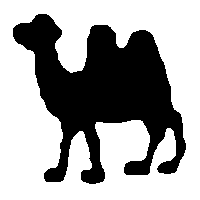
\includegraphics[width=.25\linewidth]{cheeger-2d/camel-original.png}&
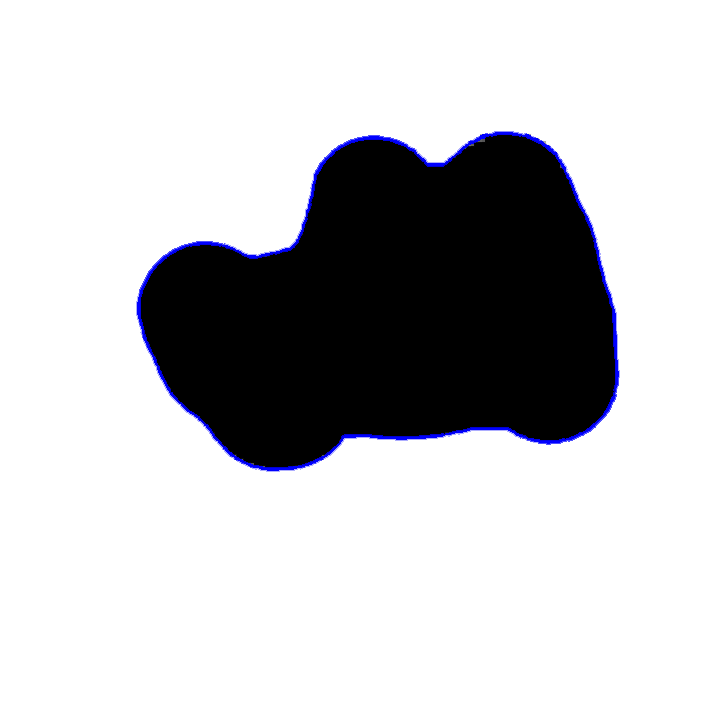
\includegraphics[width=.25\linewidth]{cheeger-2d/camel-l2-cheeger-curve.png}&

\includegraphics[width=.25\linewidth]{cheeger-2d/sapin-original.png}&
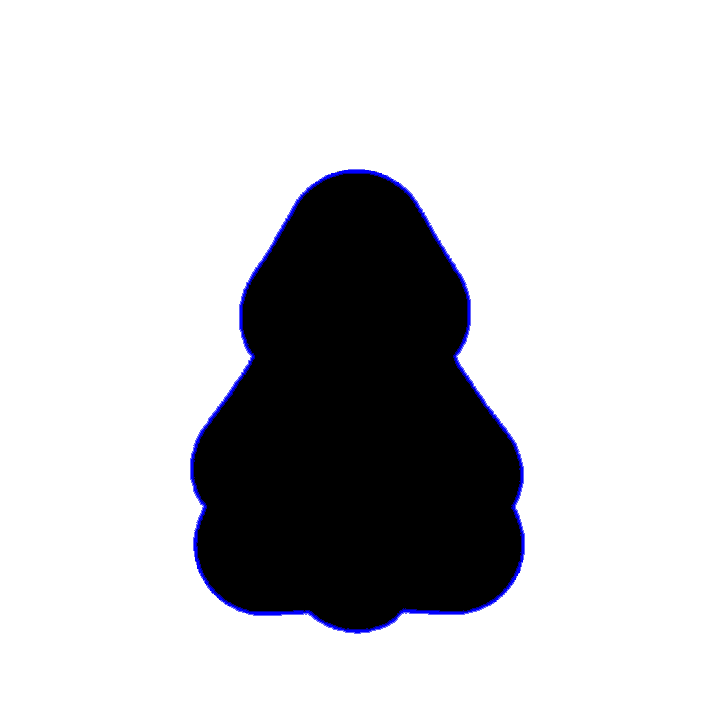
\includegraphics[width=.25\linewidth]{cheeger-2d/sapin-l2-cheeger-curve.png}
\end{tabular}
}{
Example of 2D domain $\Om$ (left) and the corresponding maximal Cheeger sets (right), computed using the method of \cite{carlier-cheeger-numeric}.
}{fig-cheeger-2d}



Our aim in the remainder of the paper is to generalize the strategy and the convergence results of \cite{carlier-cheeger-numeric} to handle the, physically more relevant, two-dimensional in-plane flow case that is detailed in the next paragraph. Of course, this two-dimensional extension presents several additional difficulties, both from a theoretical and numerical points, with respect to the unidimensional Cheeger case because of the incompressibility constraint on the one hand and the $\BD$ constraint on the other hand. 



\subsection{The in-plane case} 

In order to state the limit load problem (\ref{formerelaxee}) for  the in-plane flow case, let us set  $\DD
= \O \times \RR$ where $\O$ is a bounded domain in $\RR^2$ with a
smooth boundary $\partial \O$ divided into parts $\Gamma_0,\Gamma_1$ such that  $\Gamma_V=\Gamma_0\times \RR,  \; \Gamma_S=\Gamma_1\times \RR$.  We are looking for a  flow    in
the plane $Ox_1x_2$, i.e.  with  $v_3=0$. We put $\bv=(\bv, 0)$ (independent of $x_3$) and we will use the same notation for the   two components velocity field $\bv : \O \to \RR^2 $.   In all examples we considered that the third components body  and applied forces are vanishing ($b_{03}=f_{03} =0$). 
%% This means that  $$L(\bu)=\int_{\Gamma_1}  \bbf_0 \cdot \bu.$$  
We again use the notations $\nabla \bv$  and $\D(\bv)$ for the two dimensional gradient operator of a   two-dimensional vector field $\bv=(v_1,v_2)$ and for  its symmetric part  
\eql{ \label{eq-defn-D}
	\D(\bv) = 
	\begin{pmatrix}
		\partial_1 v_1 & \frac{1}{2}(\partial_1 v_2 + \partial_2 v_1) \\
		\frac{1}{2}(\partial_1 v_2 + \partial_2 v_1) & \partial_2 v_2
	\end{pmatrix}.
}

The  limit analysis problem  (\ref{formerelaxee}) can then be rewritten as 
\eql{\label{eq-landslide-variational}
	\frac{1}{\lambda}=\sup_{ \bu \in E, \; \Pi(\bu) \leq 1} L(\bu), 
	}
where  
$$E:=\{ \bu \in \BD(\Omega) \; ; \;    \; \dive(\bu)=0 \;   \mbox{ in  } \DD'(\O), \; \bu \cdot \bn=0 \mbox{ on } \Gamma_0 \},$$ 
 and  the plastic power $$
 \Pi(\bu) = \int_{\Omega} \kappa(x) \; d\vert \D(\bu)\vert \; (x) + \int_{\Gamma_0} g \vert \bu \vert.$$
This variational problem has exactly the form studied in paragraph \ref{mathprel} for $d=2$. This is precisely this two-dimensional case that we will treat in our numerical simulations. 

%%%%%%%%%%%%%%%%%%%%%%%%%%%%%%%%%%%%%%%%%%%%%%%

\section{Penalization scheme and convergence results}

\subsection{Convergence of the penalized scheme}


Our strategy to approximate numerically  the relaxed form of the limit load problem $\Pz$ given by (\ref{formerelaxee}) is simply to consider the following strictly concave perturbation of $\Pz$. For $\eps>0$, let us consider the penalization

 \begin{equation}\label{perturb}
\Peps \; \sup \Big \{ L_\eps(\bv) \; : \; \bv \in E, \; \Pi(\bv) \leq 1\Big\}
 \end{equation}
where 
\[L_\eps(\bv):=L(\bv)-\frac{ \eps}{d'} \int_{\DD} \vert \bv\vert^{d'}\]
where $d'=d/(d-1)$ is the conjugate exponent of the dimension $d$.  


Then, one easily gets the following: 

\begin{thm}\label{cvpenal} Under the same assumptions as in paragraph {\ref{mathprel}}, one has:
\begin{enumerate}
\item the set $\S$ of solutions of $\Pz$  is a nonempty convex and closed subset of $L^{d'}$,

\item for every $\eps>0$, $\Peps$ admits a unique solution $\bu_\eps$,

\item $(\bu_\eps)_\eps$ converges weakly in ${\rm{BD}}$ and strongly in $L^{d'}$ to $\ovu$ the element of $\S$ with minimal $L^{d'}$ norm as $\eps\to 0^+$. 

\end{enumerate}

\end{thm}


\begin{proof}
1. Nonemptyness of $\S$ has already been proved in theorem \ref{relaxts}. The fact that $\S$ is convex follows from the concavity properties of problem $\Pz$ and the fact that it is closed in $L^{d/(d-1})$ follows again from the weak compactness in $\BD$ of the admissible set of $\Pz$ and the lower semicontinuity properties described above.



\smallskip

2. Existence for $\Peps$ is exactly as in   theorem \ref{relaxts} and uniqueness follows from the strict concavity of $L_\eps$. 

\smallskip

3. Since  $\Pi(\bu_\eps)\leq 1$ for every $\eps>0$, the family $(\bu_\eps)_\eps$ is bounded in $\BD$ (and thus also in $L^{d')})$. Let then $\eps_k \to 0$ as $k\to +\infty$ be such that $(\bu_{\eps_k})_k$ weakly converges in $L^{d'}$ to some $\bu$ as $k\to \infty$. Since for every $\eps>0$ and every $\bv\in E$ such that $\Pi(\bv)\leq 1$ one has
\begin{equation}\label{inegpert}
L(\bu_\eps)-\frac{\eps }{d'} \Vert \bu_\eps\Vert_{L^{d'}}^{d'} \geq L(\bv) 
-\frac{\eps }{d'} \Vert \bv\Vert_{L^{d'}}^{d'}
\end{equation} 
taking $\eps=\eps_k$ and letting $k\to \infty$, we deduce that $\bu \in \S$. Taking $\bv=\ovu$ in (\ref{inegpert}), we then get
\[\Vert \ovu \Vert_{L^{d'}} \geq \liminf_{k }  \Vert \bu_{\eps_k} \Vert_{L^{d'}} \geq \Vert \bu \Vert_{L^{d'}}\]
so that $\bu=\ovu$ and the convergence of $\bu_{\eps_k}$ is strong in $L^{d'}$ since   $L^{d'}$ is uniformly convex. Finally, the whole family $(\bu_\eps)_\eps$ converges to $\ovu$ by standard uniqueness/compactness arguments. 


\end{proof} 

Let us remark that in the case where $\DD$ is $C^2$ and either $\Gamma_V$ or $\Gamma_S$ is empty then, using  the density result of Proposition \ref{lemdensite} (both for the intermediate and strong $L^{d'}$ topology), we deduce that the maximum in $\Peps$ is also the supremum when one restricts the maximization of $L_\eps$ to more regular test-functions: \[\sup \Peps= \sup \Big \{ L_\eps(\bv) \; : \; \bv \in E \cap C^1\cap {\rm{LD}}, \; \Pi(\bv) \leq 1\Big\}.\]

\smallskip

In our numerical examples, we will consider the case $d=2$, in this case $d'=2$ so that $\Peps$ simply amounts to project  for the $L^2$ norm $(\bb_0+\nabla f_0)/\eps$ onto  the closed and convex subset of $L^2$, $K:=\{\bv \in E, \; \Pi(\bv)\leq 1\}$. In this case, we then simply have
\[\bu_\eps={\proj_{K}} \Big( \frac{\bb_0+\nabla f_0}{\eps}  \Big).\]
Of course, the $L^2$ projection is easier to handle than the $L^{d'}$ one in general and this is why we will focus on the two-dimensional case in the sequel (although the penalization approach developed here also works in higher dimensions). 

\subsection{Convergence for the discretized problems}

% GP : Guillaume, peux tu voir pour le pbm pres des bords pour la discretization ? Je te laisse r�diger ?

%GC : ici c est ok on a pris \Gamma_V vide et donc on a une representation duale de \Pi avec des fonctions a support compact ce qui sert dans la preuve, c est clair, non?

% GP : tu utilises \DD mais ne faut  il pas plutot utiliser \Omega ?

% GC : encore une notation un peu ambigue : on utilised d abord  \DD pour le probleme en dimension quelconque puis dans le cas plan on utilise \Omega, ici on revient a la notation g�n�rique du d�but qui est \DD, c est pas g�nial mais on dit clairement que \DD est un domaine 2d, laissons comme cela


The aim of this paragraph is to prove, in dimension $2$ and  for fixed $\eps>0$, the convergence of the solution of the discretization of the penalized problem $\Peps$ to the solution of $\Peps$. As shown above,  in dimension $2$, $\Peps$ is the $L^2$ projection problem:
\begin{equation}\label{proj2d}
\inf_{u\in K} \Vert \bu -\bu^0 \Vert_{L^2}
\end{equation}
where 
\[K:=\{\bu \in E \mbox{ : } \Pi(\bu)\leq 1\}\]
and $\bu^0$ is related to the body forces, the normal traction and the penalization parameter $\eps$ via
\[\bu^0= \frac{\bb_0+\nabla f_0}{\eps}.\]
In this paragraph, the form of $\bu^0$ is not important, and one should rather think as $\bu^0$ as  an arbitrary $L^2$ vector field. The solution of (\ref{proj2d}) is denoted ${\proj_{K}}(\bu^0)$. 

\smallskip

For the sake of simplicity, we assume that $\Gamma_V=\emptyset$ (i.e. there is no Dirichlet boundary condition) and thus  that the linear form $L$ vanishes on rigid motions. For mesh size $h>0$, we discretize the smooth two-dimensional domain $\DD$ as follows. Denote by  $\DD^h$ the polyhedral domain whose closure is the union of all square cells $C_{ij}^h =[ih, (i+1)h]\times [jh, (j+1)h]$ (with $(i, j)\in \Z^2$) that intersect $\overline{\DD}$.  We then set
\[I_h:=\{(i,j)\in \Z^2 \mbox{ : } C_{ij}^h \cap \overline{\DD}\neq \emptyset\},\]
and
\[I_h^{\DD}:=\{(i,j)\in I_h \mbox{ : } C_{ij}^h, \; C_{(i-1)j}^h, \; C_{i(j-1)}^h \subset \DD\}.\]
%\; I_h^{\Gamma_0}:=\{(i,j)\in I_h \mbox{ : } C_{ij}^h \cap \Gamma_0\neq \emptyset\}.\]
Let $F_h$ denote the vector space $(\R^{2})^{I_h^{\DD}}$. For $\bu=(u^1_{ij}, u^2_{ij})_{ij}\in F_h$, partial derivatives of $\bu$ are simply discretized by finite differences
\[\partial_1^h \bu_{ij}=\frac{1}{h}(\bu_{ij}-\bu_{(i-1)j}), \; \partial_2^h \bu_{ij}=\frac{1}{h}(\bu_{ij}-\bu_{i(j-1)}),\]
as well as the divergence operator
\[
	{\dive}^{h} (\bu)_{ij}:= \partial_1^h u^1_{ij}+ \partial_2^h u^2_{ij},
\]
and the symmetrized gradient matrix
\eql{\label{eq-symgrad-disc}
	\D^h(\bu):=\frac{1}{2} \Big(\partial_k^h \bu^l+ \partial_l^h \bu ^k\Big)_{1\leq k, l\leq 2}.
}
Let us then define
\eql{\label{eq-divspace-disc}
	E_h:=\{\bu \in F_h \; : \; {\dive}^h (\bu)_{ij}=0, \; \forall (i,j)\in I_h^{\DD}\}.
}
%\bu_{ij} \cdot {\bn}_{ij}^h =0, \forall (i,j)\in I_h^{\Gamma_0}\}\]
%where ${\bn}^h_{ij}=\bn(x)$ for some $x\in \Gamma_0\cap C_{ij}^h$. 
Finally, let us define, for every $\bu\in F_h$:
\eql{\label{eq-bd-discr}
	\Pi_h(\bu):=h^2 \sum_{(i,j)\in I_h^\DD} \kappa_{ij} \vert \D^h(\bu)_{ij}\vert
}
%+h \sum_{(i,j)\in I_h^{\Gamma_0}} g_{ij} \vert \bu_{ij}\vert,\]
\[
	J_h(\bu):=h^2 \sum_{(i,j)\in I_h^\DD} \vert \bu_{ij}-\bu^0_{ij}\vert^2
\]
and
\[
	K_h:=\Big\{\bu \in E_h \; : \; \Pi_h(\bu)\leq 1\Big\}
\]
where  $\kappa_{ij}$, %$g_{ij}$ 
and $\bu^0_{ij}$ stand respectively for some discrete approximations (by mean values, say) of the data $\kappa$, 
%$g$ 
and $\bu^0$ respectively. The discretization of (\ref{proj2d}) then reads as
\begin{equation}\label{projh}
	\inf_{\bu\in K_h} J_h(\bu).
\end{equation} 	
Let then $\bu^h$ be the unique solution of the discretized projection problem (\ref{projh}) and, slightly abusing notations we shall also denote by $\bu^h$ the piecewise constant vector field with value $\bu_{ij}^h$ on the interior of the cell $C_{ij}^h$. The convergence of this scheme is then given by

\begin{thm}\label{gammacv}
	As $h\to 0^+$, $\bu^h$ converges strongly in $L^2$ and weakly in ${\rm{BD}}$ to ${\proj_{K}}(\bu^0)$, the solution of (\ref{proj2d}). 
\end{thm}
	
\begin{proof}
Since $\bu^h$ is easily seen to be bounded in $\BD$, it possesses a (not relabeled) subsequence that converges weakly in $\BD$ to some limit $\bu$.  Let us show that $\bu \in K$ i.e. 
\[\dive(\bu)=0, \; \mbox{ and } \Pi(\bu)\leq 1.\]
Let $\varphi \in C_c^1(\DD)$, setting $\varphi_{ij}:=\varphi(ih, jh)$, we first have  
\[\int_{\DD} \nabla \varphi \cdot \bu =\lim_h \sum_{(i,j)\in I_h^{\DD}}  h \Big( (u^1)^h_{ij}  (\varphi_{i+1, j}-\varphi_ {ij})+ (u^2)^h_{ij}  (\varphi_{i, j+1}-\varphi_ {ij}) \Big)\] 
and for $h$ small enough, since $\varphi$ has compact support in $\DD$ and since $u^h \in E_h$,  the latter sum equals
\[-h\sum_{(i,j)\in I_h^{\DD}} {\dive}_h (\bu^h)_{ij} \varphi_{ij}=0\]
so that $\dive(\bu)=0$. To prove that $\Pi(\bu)\leq 1$, we use the representation formula
\[\Pi(\bu)=\sup  \Big\{\int_{\DD} \bfdiv(\bs) \cdot \bu \; :  \bs \in C_c^1(\DD, \S_2), \; \vert \bs \vert \leq \kappa  \Big\}\]
we then take $\bs \in C_c^1(\DD, \S_2)$ such that $\vert \bs \vert \leq \kappa$ pointwise and discretize $\bs$ at points $(ih, jh)$ by values $\bs_{ij}$ such that $\vert \bs_{ij}\vert\leq \kappa_{ij}$, we then have
\[\begin{split}
\int_{\DD} \bfdiv(\bs) \cdot \bu&=-\lim_h  \sum_{(i,j)\in I_h^{\DD}}  h^2  \D^h(\bu^h)_{ij} : \bs_{ij}\\
&\leq \limsup \sum_{(i,j)\in I_h^{\DD}}  h^2  \kappa_{ij} \vert \D^h(\bu^h)_{ij}\vert  \\
&=\limsup \Pi_h (\bu^h)\leq 1.
\end{split}\]
Which proves that $\bu \in K$. 


\smallskip

Now let $\bv=(v_1,v_2) \in  K \cap C^1(\DD)\cap {\rm{LD}}$ and define the discretization , $\bv^h=((v^1)^h, (v^2)^h)$ by
\[(v^1)^h_{ij} :=h^{-1} \int_{h[(i, j-1), (i,j)]} v_1, \; (v^2)^h_{ij} :=h^{-1} \int_{h[(i-1, j), (i,j)]} v_2\]
since $\bv$ is divergence-free, its flux through $\partial C_{ij}^h$ is zero and then $\bv^h\in E_h$. Let $\delta>0$ since $\bv\in C^1(\DD)\cap {\rm{LD}}$, it easily follows from Lebesgue's dominated convergence theorem that
\[\lim_h \Pi_h(\bv^h)= \Pi(\bv) \leq 1 \]
hence $(1+\delta)^{-1} \bv^h\in K_h$ i.e. is admissible for (\ref{projh}) for $h$ small enough. We thus have 
\[F_h(\bu^h)\leq F_h\Big(\frac{\bv^h}{1+\delta}\Big)\]
letting $h\to 0^+$, we thus have
\[\Vert \bu -\bu^0\Vert_{L^2} \leq \Big\Vert \frac{\bv}{1+\delta} -\bu^0\Big\Vert_{L^2}\]
letting $\delta\to 0^+$, we deduce that 
\[\Vert \bu -\bu^0\Vert_{L^2} \leq \Big\Vert \frac{\bv}{1+\delta} -\bu^0\Big\Vert_{L^2},  \;  \forall \bv \in K \cap C^1(\DD)\cap {\rm{LD}}\]
and we thus conclude from proposition \ref{lemdensite} that $\bu=\proj_{K}(\bu^0)$. By standard compactness/uniqueness argument, the whole sequence $(\bu^h)$ thus converges to $\proj_{K}(\bu^0)$ weakly in $\BD$. Finally, strong $L^2$ convergence comes from
\[ \Vert \bu^h -\bu^0 \Vert_{L^2} \to \Vert \bu -\bu^0 \Vert_{L^2}  \mbox{ as } h\to 0^+\] 
and the uniform convexity of $L^2$. 
\end{proof}	
		
The case where $\Gamma_V\neq \emptyset$ is not covered by the previous convergence result. In this more general case, one has two extra difficulties : discretizing in a consistent way the boundary conditions and the density in energy of smooth functions (which was a crucial point in the previous proof). Again, when $\DD$ is a rectangle and $\Gamma_V$ consists of its vertical boundary, these difficulties may be overcome. 

%%%%%%%%%%%%%%%%%%%%%%%%%%%%%%%%%%%%%%%%%%%%%%%%
%%%%%%%%%%%%%%%%%%%%%%%%%%%%%%%%%%%%%%%%%%%%%%%%
%%%%%%%%%%%%%%%%%%%%%%%%%%%%%%%%%%%%%%%%%%%%%%%%
\section{Numerical computation of limit load}		

This section describes a numerical scheme to solve the discretized version \eqref{projh} of the limit load approximation problem \eqref{proj2d}. This scheme solves an unconstrained dual optimization problem using an accelerated first order algorithm.



%%%%%%%%%%%%%%%%%%%%%%%%%%%%%%%%%%%%%%%%%%%%%%%%%%%%%%%%%%%%%%%
\subsection{Dual unconstrained problem}

% projector onto div=0 space
\newcommand{\projE}{{\boldsymbol P}}

The following proposition shows that the discretized projection $\bu^h$ that solves \eqref{projh} can be computed by solving an unconstrained dual optimization problem. This dual optimization extends the result of \cite{FadiliTV} that was used to compute the projection of an image on a total variation ball.



\begin{thm}
	The solution $\bu^h$ of \eqref{projh} satisfies
	\eq{
		\bu^h = \projE^h( \bu^0 - \D^{h*}(\bs^h) ),
	} 
	where $\bs_{ij}^h \in \RR^{2 \times 2}$ is a solution of
	\eql{\label{eq-dual}
		\umin{\bs}
		 J(\bs) = \frac{1}{2} \norm{ \projE^h( \bu^0 - \D^{h*}(\bs) ) }^2 + \normi{ \bs }
	}
	where $\D^{h*}$ is the operator dual to $\D^h$ defined in \eqref{eq-symgrad-disc},
	$\projE^h$ is the orthogonal projector on the space $E_h$ defined in \eqref{eq-divspace-disc}, 
	and the $\linf$ norm of a tensor field $\bs_{ij} \in \RR^{2 \times 2}$ reads
	\eq{	
		\normi{ \bs } = \umax{ (i,j) \in I_h^{\DD} } \kappa_{ij}^{-1} |\bs_{ij}|.
	}
\end{thm}
\begin{proof}
	Introducing dual variables $\bs_{ij} \in \RR^{2 \times 2}$, one can write the indicator function of the BD unit ball as
	\eq{
		1_{\Pi_h(\cdot) \leq 1}(\bu) = \umax{\bs} \dotp{\bs}{\D^h \bu} - \normi{\bs}
		= \choice{
			0 \qifq \Pi_h(\bu) \leq 1, \\
			+\infty \quad \text{otherwise},
		},
	}
	where the discrete BD norm is defined in \eqref{eq-bd-discr}.
	This allows one to rewrite \eqref{projh} as 
	\eql{\label{eq-proof-dual-1}
		\umax{\bs}  - \normi{\bs}
		+ \umin{ \bu \in E_h } \dotp{\bs}{\D^h \bu} + \frac{1}{2}\norm{\bu-\bu^0}^2.
	}
	The inner minimization is solved using the projector $\projE^h$ as
	\eq{
		\bu^h = \uargmin{\bu \in E_h} \dotp{\bs}{\D^h \bu} + \frac{1}{2}\norm{\bu-\bu^0}^2
		= \projE^h( \bu^0 - \D^{h*} \bs  ),
	}
	and
	\eql{\label{eq-proof-dual-2}
		\dotp{\bs}{\D^h \bu} + \frac{1}{2}\norm{\bu^0-\bu}^2
		= - \frac{1}{2}\norm{ \projE^h(\bu^0 - \D^{h*} \bs) }^2+c
	}
	where $c$ is a constant that does not depends on $\bs$.
	Combining equations \eqref{eq-proof-dual-1} and \eqref{eq-proof-dual-2}
	leads to the optimization \eqref{eq-dual}.
\end{proof}

%%%%%%%%%%%%%%%%%%%%%%%%%%%%%%%%%%%%%%%%%%%%%%%%
\subsection{Dual minimization algorithm}

To ease notations, we drop the dependency on the grid size $h$ in the remaining part of the paper. 

Several iterative first order schemes exist to minimize \eqref{eq-dual}, which is a sum of a smooth functional $\norm{ \projE(\bu^0 - \D^* \bs) }^2$ and a non-smooth functional $\normi{\bs}$.

%%%
\paragraph{Proximal operator.}

The non-smooth part $\normi{\bs}$ of the functional is regularized during the iteration of a first order scheme by computing the proximal operator, for some $\rho > 0$,
\eql{\label{eq-proximal-inf}
	\Prox_{\rho  \normi{\cdot}}(\bs) = 
	\uargmin{\tilde \bs} \frac{1}{2} \norm{\tilde \bs - \bs}^2 + \normi{\tilde \bs}.
}

Proposition \ref{prop-soft-thresh} shows that the proximal operator defined in \eqref{eq-proximal-inf} is computed explicitly using a soft thresholding $S_\la$ for a well chosen value of $\la$. 

Computing the precise value of $\la$ for a given matrix field $\bs_{ij} \in \RR^{2 \times 2}$ requires the computation of $d_0 \leq d_1 \leq \ldots \leq d_{N-1}$ that orders the set of norms
\eql{\label{eq-def-d}
	\{d_t\}_{t=0}^{|I_h^{\DD}|} = \{ |\bs_{ij}| \}_{ (i,j) \in I_h^{\DD}}, 
}
and also the cumulated ordered norms
\eql{\label{eq-def-D}
	D_s = \sum_{t=s+1}^{N-1} d_t.
}

\begin{prop}\label{prop-soft-thresh}
	For $\bs_{ij} \in \RR^{2 \times 2}$, one has 
	\eq{
		\Prox_{\rho \normi{\cdot}}( \bs ) = \bs - S_\la(\bs)
	} 
	where
	\eql{\label{eq-soft-thresh}
		S_\la( \bs )_{ij} = \max\pa{ 1 - \frac{\la \kappa_{ij}}{ |\bs_{ij}| } , 0 } \bs_{ij}
	}
	and $\la > 0$ is computed as 
	\eql{\label{eq-defn-la}
		\la = d_t + (d_{t+1}-d_t) \frac{D_{t+1} - \rho}{ D_{t+1} - D_t }
	}
	where $d$ and $D$ are defined in \eqref{eq-def-d} and \eqref{eq-def-D}, and where 
	$t$ is such that $D_{t+1} \leq \rho  < D_t$.	
\end{prop}
\begin{proof}
The resolution of \eqref{eq-proximal-inf} is computed using the relationship between the proximal operator of the norm $\normi{\cdot}$ and the projection on the dual norm $\normu{\cdot}$, see \cite{combettes-proximal},
\eq{
	\Prox_{\rho \normi{\cdot}}( \bs ) = \bs - \Proj_{\normu{\cdot} \leq \rho}(\bs)
}
where the $\lun$ norm is defined as
\eq{
	\normu{\bs} = \sum_{(i,j) \in I_h^{\DD} } \kappa_{ij} |\bs_{ij}|.
}
and where $\Proj_{\normu{\cdot} \leq \kappa}(\bs)$ is the orthogonal projection of $\bs$ onto the set $\enscond{\bs}{\normu{\bs} \leq \rho}$
\eq{
	\Proj_{\normu{\cdot} \leq \rho}(\bs) = \uargmin{\tilde \bs, \, \normu{\tilde \bs} \leq \rho } \norm{\bs-\tilde \bs}.
}

The projection $\Proj_{\normu{\cdot} \leq 1}(\bs)$ is computed by noticing that it is the solution of a regularized minimization
\eq{
	\Proj_{\normu{\cdot} \leq \rho}(\bs) = \uargmin{ \tilde \bs } \frac{1}{2} \norm{\bs-\tilde \bs}^2 + \la \normu{\tilde \bs}.
}
for a well chosen value of $\la > 0$.

As noticed for instance in \cite{chambolle-wavelets} for wavelet thresholding, the solution of such a $\lun$ regularized is computed using a soft thresholding
\eq{
	\Proj_{\normu{\cdot} \leq 1}(\bs) = S_\la(\bs).
}
One can then check that the value \eqref{eq-defn-la} of $\la$ ensure that $\norm{S_\la(\bs)} = \rho$.
\end{proof}



%%
\if 0
\paragraph{Single-step First Order Scheme}

The simplest method to solve \eqref{eq-dual} is to compute forward-backward iterates $\sik$ that generalize a projected gradient descent using the proximal operator
\eql{\label{eq-proximal-iter}
	\bs^{(k+1)} = \Prox_{ \mu \normi{\cdot}}( \sik - \mu \D P (\bu^0 - \D^* \sik) ).
}
If $\mu < 2/\norm{\D \D^*} = 1/8$, one can prove the convergence of this scheme to a minimizer of \eqref{eq-dual}, see for instance \cite{combettes-proximal}.
\fi

%%
\paragraph{Multi-step First Order Scheme}


\newcommand{\sik}{\bs^{(k)}} 

Y. Nesterov in \cite{nesterov-gradient,nesterov-smooth} proposes a first order scheme to find a minimizer $\bs^h$ of functional of the form $J(\bs)$ as defined in \eqref{eq-dual}. It computes iterates $\sik$ that converge to a solution $\bs^h$ using a multi-steps generalized gradient descent that makes use of previous iterates $\bs^{(i)}$, $i < k$ to compute $\sik$. 

For a restricted set of non-smooth functionals, such as the functional $J$ minimized in \eqref{eq-dual}, he shows that this method reaches the energy decay lower bound 
\eql{\label{eq-decay-dual}
	J(\sik)-J(\bs^\star) = O(1/k^2)
}
achievable by first order schemes. This method have found many applications recently in image processing, see for instance  \cite{weiss-tv-nesterov, FadiliTV}.

Table \ref{algorithm-tv-proj-nesterov} details the steps of Nesterov scheme to minimize \eqref{eq-dual}. The step size $\mu$ should satisfy $\mu < 2/\norm{\D \D^*}$ for the method to converge. This algorithm is an extension of the algorithm of Fadili and Peyr\'e \cite{FadiliTV} that computes the projection on a ball of image with bounded variation. Our algorithm considers instead vector fields with bounded deformation, and includes a divergence free constraint that makes the computations more difficult.

A slight generalization of the result in \cite{FadiliTV} shows that not only one has a fast decay \eqref{eq-decay-dual} on the objective function $J$, but also on the primal iterates, which is more interesting for our application.

\begin{thm}
	If $\mu < 2/\norm{\D \D^*}$, the iterates $\bu^{(k)} = \projE( \bu^0 - \D^* \bs^{(k)})$ computed with the algorithm of Table \ref{algorithm-tv-proj-nesterov} satisfy
	\eq{
		\norm{ \bu^{(k)}-\bu^h }^2 = O(1/k^2)
	}
	where $\bu^h$ is the solution of \eqref{projh}.
\end{thm}
\begin{proof}
 	A similar result for the projection on the total variation ball has been proved in \cite{FadiliTV}  (without linear constraints). The proof of \cite{FadiliTV} adapts directly to our situation. 
\end{proof}

\newcommand{\g}{{\boldsymbol \al}}
\newcommand{\z}{{\boldsymbol \be}}
\newcommand{\y}{{\boldsymbol \ga}}

\begin{algorithm}
\noindent{\bf Initialization:} set $\bs^{(0)}_{ij}=0 \in \RR^{2 \times 2}$, $k=0$, $A=0$, $\g^{(0)}_{ij} = 0 \in \RR^{2 \times 2}$ \;
\Repeat{$\norm{\bs^{(k+1)} - \bs^{(k)}} \leq \tol$}
{
\begin{itemize}
	\item \textit{First proximal computation:} compute 
	\eq{
		\z^{(k)} = \Prox_{A \normi{\cdot}}( \bs^{(0)} - \g^{(k)} )		
	}
	where the proximal operator is computed as defined in Proposition \ref{prop-soft-thresh} with $\rho=A$.
	Set $a = (\mu + \sqrt{\mu^2 + 4\mu A})/2$.
	\item \textit{Second proximal computation:} compute
	\begin{align*}
		\y^{(k)} &= \frac{ A \sik + a \z^{(k)} }{ A + a },\\
		\tilde \y^{(k)} &= \y^{(k)} + \frac{\mu}{2} \D P ( \bu^0 - \D^* \y^{(k)} ),\\
		\bs^{(k+1)} &= \Prox_{\mu / 2 \normi{\cdot}}( \tilde \y^{(k)} ).
	\end{align*}
	where the proximal operator is computed as defined in Proposition \ref{prop-soft-thresh} with $\rho=\mu / 2$.
	\item Set $A \leftarrow A+a$, 
		\eq{
			\g^{(k+1)} = \g^{(k)} - a \D \projE( \bu^0 - \D^* \bs^{(k+1)} ),
		} 
		and $k \leftarrow k+1$.
\end{itemize}
}
\noindent{\bf Return:} the projection 
$\bs^h = \projE( \bu^0 - \D^* \bs^{(k+1)})$. 
    \caption{Multi-step dual projection. \label{algorithm-tv-proj-nesterov}}
\end{algorithm}

The main computational bottleneck of the algorithm is the computation of the projection $\projE$ on the set $E_h$ of divergence free vectors. In practice, this projection is computed approximately using a conjugate gradient descent. This projection should be computed with high enough precision to avoid convergence issues. In practice, one can use a warm restart and use the previous iterate as an initialization for the conjugate gradient, so that only a few steps are required at each iteration.


%%
\paragraph{Discussion about the numerical scheme.}

We note that one could use other first order schemes to perform the minimization \eqref{eq-dual}.
In particular, Beck and Teboulle propose in \cite{beck-fista} a first order scheme that enjoys the same energy decay \eqref{eq-decay-dual} but is simpler to implement and is more stable to the imperfect computation of the projection.

Instead of performing the strictly convex relaxation \eqref{proj2d}, one can also tackle directly the original convex problem \eqref{formerelaxee}. This requires the maximization of a linear form under bounded deformation and incompressibility constraints. A careful re-writing of the problem makes it tractable using an ``alternative direction method of multipliers'', as described in \cite{eckstein-dr}. Similarly to our algorithm, each iteration of such a scheme requires the computation of the proximal operator and a projection on an incompressibility constraint. 

% Gabriel : on peut mettre un truc du style si vous voulez : 

% An advantage of our scheme is that one has a speed of convergence, and it captures approximately . It is however beyond the scope of this paper to compares the numerical merits of each method

%%%%%%%%%%%%%%%%%%%%%%%%%%%%%%%%%%%%%%%%%%%%%%%%
%%%%%%%%%%%%%%%%%%%%%%%%%%%%%%%%%%%%%%%%%%%%%%%%
%%%%%%%%%%%%%%%%%%%%%%%%%%%%%%%%%%%%%%%%%%%%%%%%
\section{Numerical results}		
	
We present here some  numerical simulations for three important limit load problems (two notched tensile, indentation and porous metals).   For all  numerical experiments, we have used a finite grid of $200 \times 200$ points, and the  approximation parameter was chosen to be $\epsilon=\Pi^h(\nabla f_0)/100$.
		
%%%%%%%%%%%%%%%%%%%%%%%%%%%%%%%%%%%%%%%%%%%%%%%%%%%%%%%%%%%%%%%%%%%%%%%%%%%%%
\subsection{Two Notched Tensile Problem}

 The two notched tensile problem  is a popular benchmark test used for rigid-plastic and elasto-plastic analysis which was   introduced by Nagtegaal et al. \cite {NPR} to illustrate locking.  The structure depicted in Figure \ref{fig-notched-pbm} (left) consists of a rectangular  specimen of length $2$ with two thin notches under an  in-plane tensile load $\tau_0$.  Using the above notations we put $\Gamma_0=\emptyset, \Gamma_1=\partial \O$ and $\bbf_0=(0,\tau_0)$ on the right side, $\bbf_0=(0,-\kappa)$ on the left side.  The yield limit  is constant  $\kappa=\sqrt{2}\tau_0$ and the body forces are vanishing ($\bb =0$), which means that $ L(\bu)=\int_{\Gamma} \bbf_0 \cdot \bu \; d\Gamma$. We considered here only the case $a=1$.  
 
 
 \myfigure{
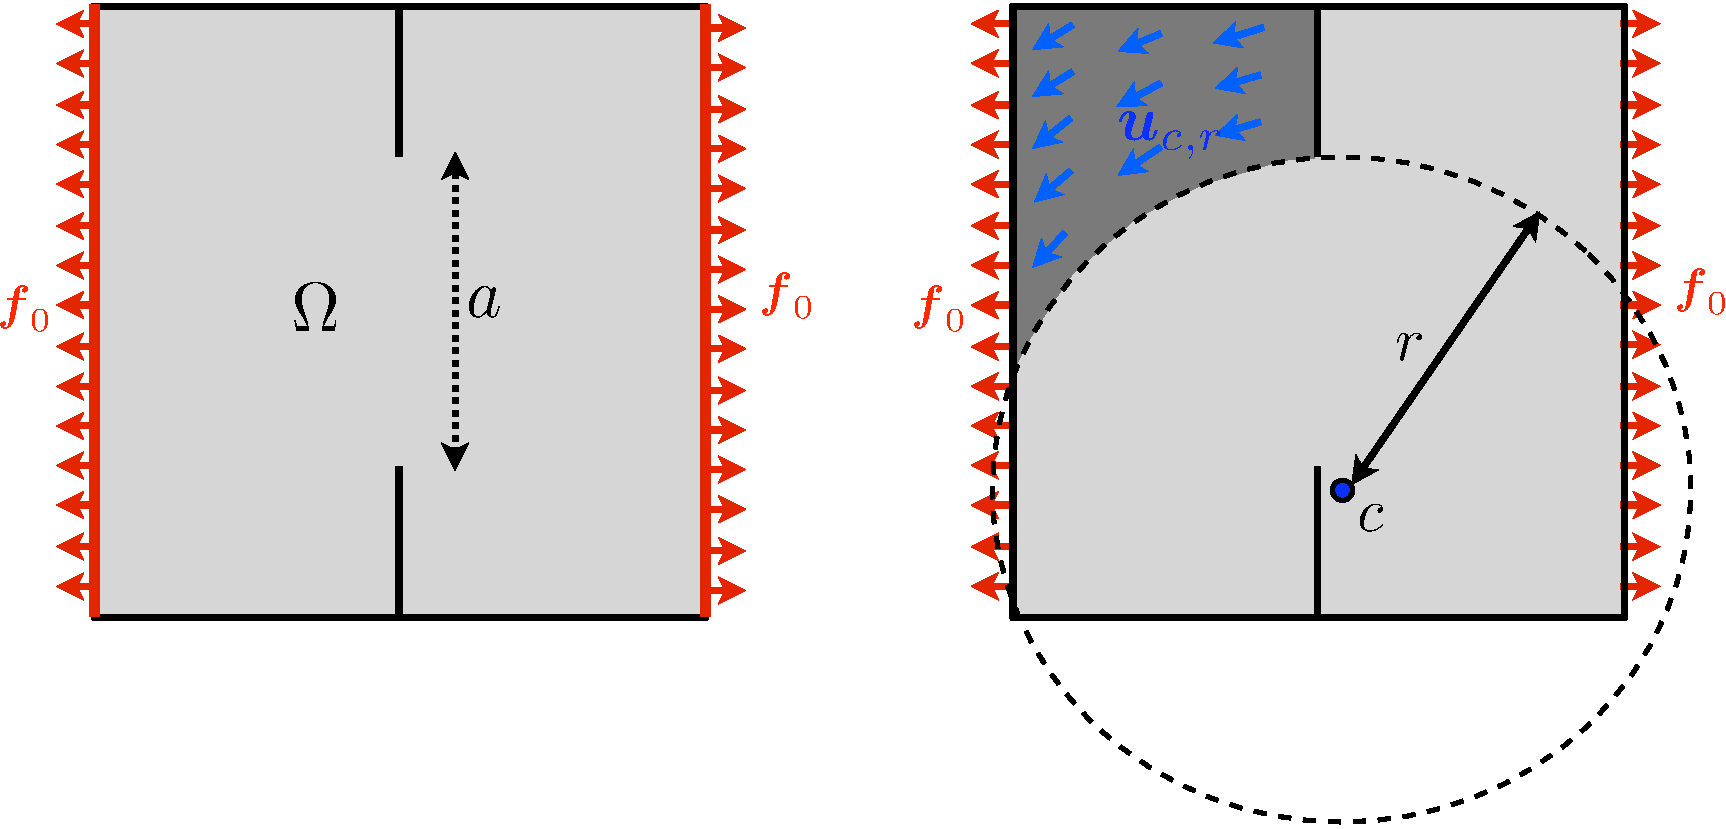
\includegraphics[width=.95\linewidth]{notched/notched-pbm.pdf}[ht]
}{
Left: schematic view of the two notched tensile problem.
Right: semi-analytical solution obtained with DVDS   \cite{IO}.
}{fig-notched-pbm}


 
 
 The "reference" value  provided by Christiansen 
and Andersen \cite{CA} and widely considered to be extremely accurate is $\lambda\approx1.136$.  The  same value was found  by Ionescu and Oudet \cite{IO}  with the  discontinuous velocity domain splitting (DVDS) method. The corresponding fracture configurations are plotted in Figure \ref{fig-notched-pbm} (right).  DVDS uses a parametric family of vector field $\bu_{c,r}$ parameterized by a center $c \in \RR^2$ and a radius $r>0$, see an example in Figure \ref{fig-notched-pbm}, right. The vector field $\bu_{c,r}$ corresponds to rotation movement outside the circle of center $c$ and radius $r$ and DVDS computes   optimal parameters $(c,r)$ (see \cite{IO})  and they found 
\eq{
	\la \leq \la(\bu_{c,r}) =  \frac{ \Pi(\bu_{c,r}) }{L(\bu_{c,r})} \approx 1.136.
}
This result, obtained without any finite element discretization,   is more accurate  than   $\lambda \approx  1.166$ obtained by Tin-Loi and Ngo  \cite{TN} using a $p$-version finite element method  ($p = 15$).   



Figure \ref{fig-notched-numerics}, left, shows the solution $\bu^h$ computed with our algorithm. The arrows shows some vectors $\bu^h_{ij}$, and the color maps indexes the red (resp. blue) channel using the X (resp. Y) value of the vector field. Colors allows one to better visualize the discontinuities in the vector field. The numerical constant computed with our algorithm is 
\eq{
	\la(\bu^h) =  \frac{ \Pi(\bu^h) }{L(\bu^h)} \approx 1.094. 
}
This value is slightly smaller than the value computed in \cite{IO} and  \cite{CA}. 

%This might be because our algorithm is able to compute a solution over the whole domain $\Om$, whereas the solution $\bu_{c,r}$ is localized only on subset of the domain.

\myfigure{
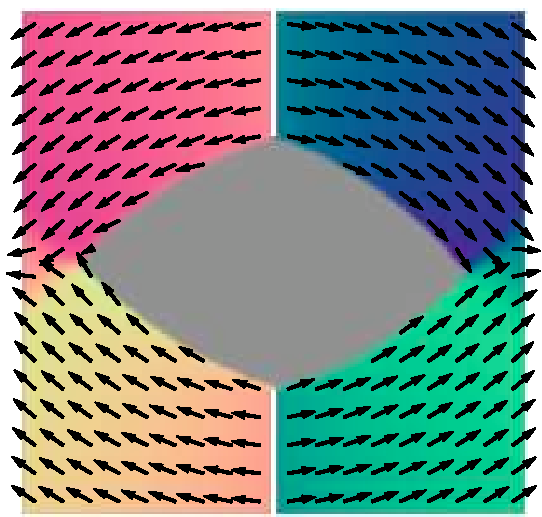
\includegraphics[width=.6\linewidth]{notched/notched-numerics-rotated.pdf}
}{
	Numerical solution $\bu^h$ computed with our algorithm for the two notched tensile problem.
}{fig-notched-numerics}



%%%%%%%%%%%%%%%%%%%%%%%%%%%%%%%%%%%%%%%%%%%%%%%%%%%%%%%%%%%%%%%%%%%%%%%%%%%%%
\subsection{Indentation Problem}

In this problem, we consider  a half space, that is handled numerically as an infinite rod  with a  elongated rectangle $\Om$ section. The loading force $\bbf_0$ is localized on a small segment $[A,B]$ of the upper boundary of the rod. Dirichlet condition $\bv=0$ are imposed on the lower boundary $\Ga_V$ of $\Om$. The yield limit $\kappa=1$ is constant within the road. Figure \ref{fig-indentation-pbm}, left, shows the setting for this numerical experiment.


Two  explicit vector fields $\bv$ have been proposed  by Hill and by Prandtl to find an upper estimation  for  $\la$ (see for instance \cite{K}). They all give the same value 
\eql{\label{eq-indentation-lambda}
	\la \leq \la(\bv) = \frac{ \Pi(\bv) }{ L(\bv) } = \frac{2+\pi}{\sqrt{2}} \approx 3.64.
}
%To the best of our knowledge, it is unknown if this upper bound is in fact the true value of $\la$.
Figure \ref{fig-indentation-pbm}, right, shows such an explicit solution, proposed by Prandtl (see \cite{K}). It is constant over three orthogonal triangles $(ABE)$, $(BCF)$, $(CGD)$ and corresponds to a rotation over the two quarter of discs $(BEF)$, $(CFG)$.

\myfigure{
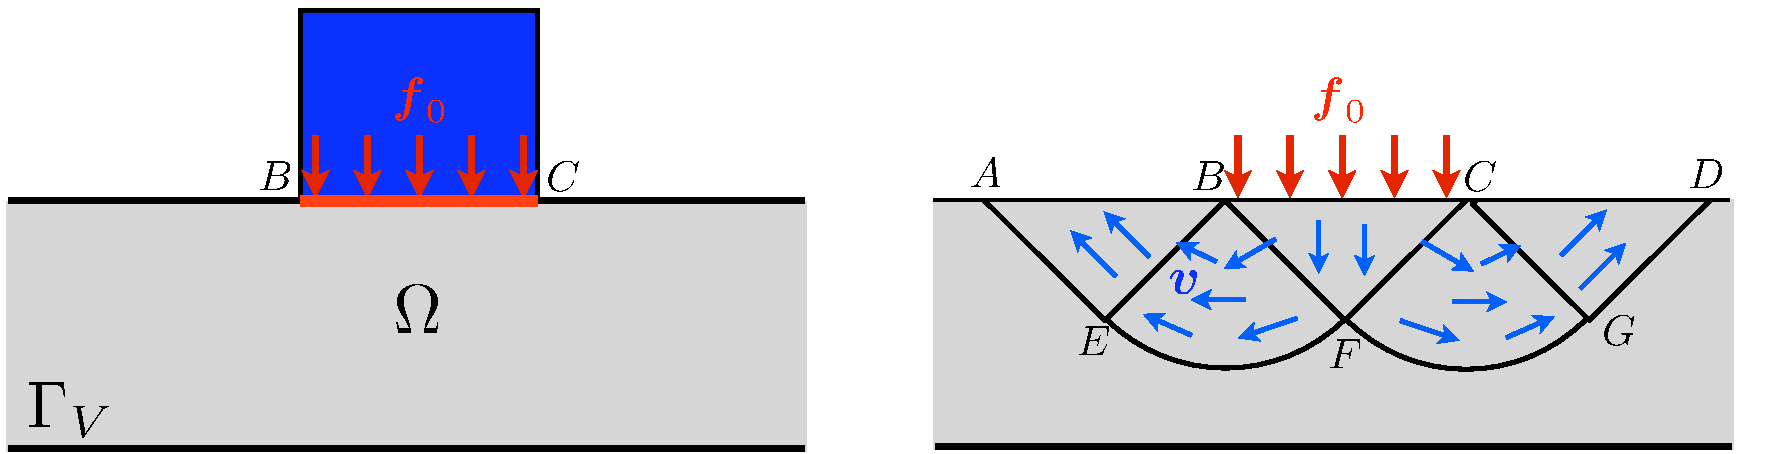
\includegraphics[width=.95\linewidth]{indentation/indentation-pbm.pdf}
}{
Left: schematic view of the indentation problem.
Right: analytical solution of Prandtl.
}{fig-indentation-pbm}

Figure \ref{fig-indentation-numerics}, right, shows the solution $\bu^h$ computed with our algorithm. The numerical constant computed with our algorithm is 
\eq{
	\la(\bu^h) =  \frac{ \Pi(\bu^h) }{L(\bu^h)} \approx 3.79.  % OLD VALUE : 3.85 
}
This value is close but slightly larger than the value computed using the explicit solutions in \eqref{eq-indentation-lambda}, which shows that there is still room for improvements. 

%Reaching better values by decreasing the step size $h$ or the approximation parameter $\epsilon$ appears to be too demanding numerically with our method. 

\myfigure{
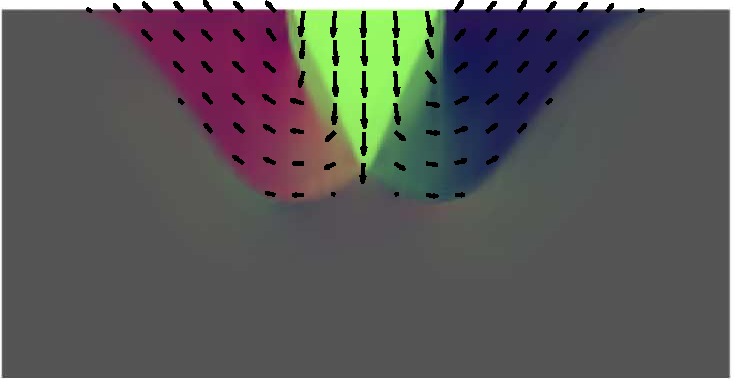
\includegraphics[width=.7\linewidth]{indentation/indentation-numerics-new}
}{
	Numerical solution $\bu^h$ computed with our algorithm for the  indentation problem.
}{fig-indentation-numerics}


%%%%%%%%%%%%%%%%%%%%%%%%%%%%%%%%%%%%%%%%%%%%%%%%%%%%%%%%%%%%%%%%%%%%%%%%%%%%%
\subsection{Compression of porous metals}


The ductile failure of porous metallic materials are usually  studied  using the lower and upper bound methods of limit load analysis.  
For cylindrical and spherical cavities, the  problem wad firstly treated by Gurson with his famous kinematical approach \cite{G77}, which gives an analytical upper bound  of the homogenized yield criterion.  There are lots of numerical  approaches, using various limit load techniques (see for instance \cite{TP,Fal,Bal})  which confirmed and corrected the original Gourson model. 

We want to illustrate here how our numerical method can be used  to compute the  limit load  for  metals with cavities.  For  that we consider  $\Omega$ to be  a square of unit side length, with a smaller square hole  of side length $1/3$. The yield limit $\kappa=1$ is constant within $\Om$ and the loading force (see Figure \ref{fig-gurson} left) is  $\bbf_0=-\frac{1}{2}\bn$ on the left and the right sides and   $\bbf_0=-\frac{\sqrt{3}}{2}\bn$,  on the upper and bottom sides (here 
%\eq{
%	\bbf_0(x) = 
%	\begin{pmatrix}
%		\cos(\th) & 0\\
%		0 & \sin(\th)
%	\end{pmatrix}
%	n(x).
%/}
 $\bn$ is the exterior normal to the external boundary).   In Figure \ref{fig-gurson} right we have plotted the numerical solution computed with our algorithm.  We remark that the algorithm is able to capture the presence of two symmetric  discontinuities(fractures) in the velocity field.  
The value of the constant computed with our algorithm is $\la(\bu^h) = 1.315$.


\myfigure{
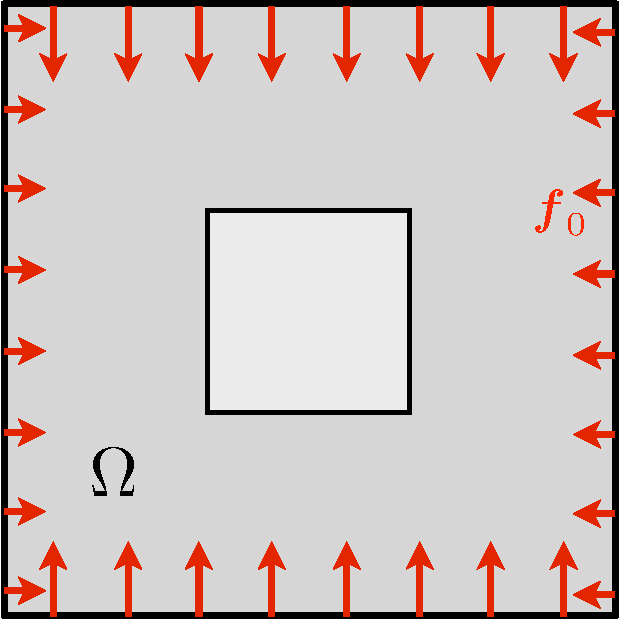
\includegraphics[width=.4\linewidth]{gurson/gurson-pbm.pdf}\hspace{3mm}
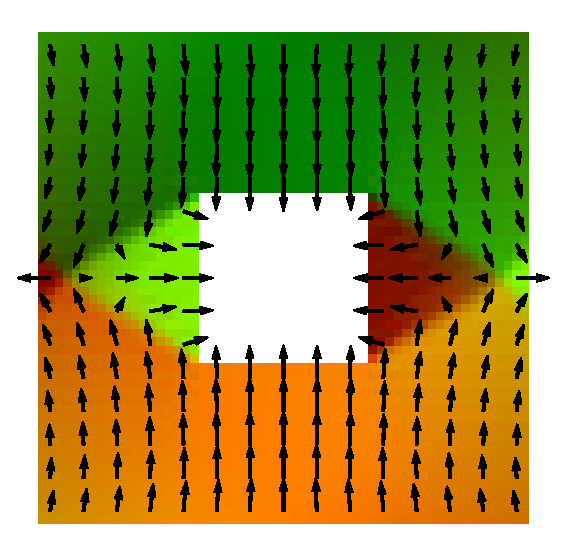
\includegraphics[width=.44\linewidth]{gurson/gurson-numerics.eps}
}{
Left: plane-strain compression of  a square  with a square void.
Right: numerical solution computed with our algorithm.
}{fig-gurson}


\section*{Acknowledgments}

The authors would like to thank Jalal Fadili for his help during the development of the numerical scheme. G.C.  gratefully acknowledges the support of the Agence Nationale de la Recherche through the project  ``ANR-07-BLAN-0235 OTARIE''.



%%%%%%%%%%%%%%%%%%%%%%%%%%%%%%%%%%%%%%%%%%%%%%%%%%%%%
%%%%%%%%%%%%%%%%%%%REFERENCES%%%%%%%%%%%%%%%%%%%%%%%%

\bibliographystyle{plain}  % plain alpha
\bibliography{bibliography}		
		

\end{document}
